\chapter{Training, Testing and Hyperparameters Tuning of a Multi-class
Vehicle Classifier}
\label{Chapter 4}
As mentioned in earlier chapters, CNNs are predominantly used for
image classification and detection in pattern recognition and
computer vision problems. Recall that classification is the process of putting a tag on
an image from a set of class labels. This chapter describes in detail
the process of designing, training, testing and hyper-parameters
tuning of a a five-class image classifier. The following sections
cover in detail the step-by-step process of training a five-class vehicles
classifier. Furthermore, results are tabulated as values of
hyper-parameters are changed to achieve better test accuracy and reduced
classification loss.
\section{Formation of Dataset}
Deep learning based image classification works by inputting class
image examples to a CNN; CNN is then trained for higher test accuracy
and reduced test loss. The set of images used for this purpose is
called a dataset.
The dataset is divided into training and test dataset by a specific ratio.
In this project we have five different classes of vehicles i.e. Bus, Car, Truck, Motorcycle
and Hiace. There are a total of 10000 images with 2000 images of each 
class. These images are downloaded from Google search results and from already available
datasets and from websites providing licensed free images like Flickr.
APIs along with Python
scripts can be used to download these images from the internet.
Using matplotlib in python, we can plot some of the images with the output as
shown in listing \ref{listing:4.1} and plot is attached in figure
\ref{fig:4.1}.
\linespread{1.0}
\begin{listing}[H]
\begin{minted}[bgcolor=bg,
    linenos = true,
    xleftmargin=20pt,
    framesep = 2mm]{python}
import matplotlib.pyplot as plt
from matplotlib.image import imread  
path  = './images/'
for i in range(9):
    plt.subplot(330+1+i)
    filename = path + 'image_'+ str(i) + '.jpg'
    image = imread(filename)
    plt.imshow(image)    
    plt.show()
\end{minted}
\caption{Python script to plot some images from each class}
\label{listing:4.1}
\end{listing}

\begin{figure}[H]
    \centering
    \captionsetup{justification = centering}
    \includegraphics[scale = 0.8]{CHAPTERS/Chapter-4/Images/4.1.png}
    \caption{Plot of some images from each class} 
    \label{fig:4.1}
  \end{figure}

\subsection{Data Augmentation}
Training deep learning CNN architectures on larger datasets
results in more skillful models and improved classification accuracy.
However, availability of large amount of  class-specific data is a challenge.
This problem of lack of sufficient data can be solved using
techniques which expand the size of available data by introducing
modifications and variations by performing image manipulation.
Dataaugmentation is the process of applying techniques like shifting, 
flipping, rotating and varying the brightness etc on images to
introduce variations in images. The Keras deep learning NN library uses
ImageDataGenerator
class to achieve image data augmentation and is used in our code.

\section{Setting of Workspace for the Project}
There are a lot of images to be processed. To process images, high end GPU is
needed. Due to unavailability of an Nvidia GPU on the system, we used Google Colab.
It is an online platform having high end GPUs free provided by Google for training
up to 12 hours. Enabling a GPU in the notebook settings can accelerate the process of
training.
\section{Designing and Training of DCNN for Multi-Class Classification}
In our project we have used Keras for designing, training and testing of 
DCCN architectures for our multi-class classification problem.
Keras is one of the leading high level API for neural networks. It contains
many modules such as layers, cost functions, activation functions, initialization
schemes and regularization schemes. This project uses Keras for training purposes.
\subsection{Conversion of Images and Labels to Numpy Arrays}
After importing all the necessary packages, we are all set to pre-process our data.
Recall to chapter 2, where we studied the basics of an image. In Keras, an image has two
representations i.e. (width, height, color\_channels) and (color\_channels, width, height).
First approach is called as ``channels first approach" and
the latter is called as ``channels last approach".
We will use the ``channels last approach".

First step is to read the images from the folder mounted from Google drive.
Labels are assigned to classes from 0 to 4. Keras load\_img() routine loads image
from the folder with given target size. Target size for this project is chosen as
$128 \times 128$. This means that both width and height has a size of 128 pixels.
There are 3 color channels for RGB images. Images are then converted to numpy arrays using
Keras img\_to\_array() method. Labels are stored as 0, 1, 2, 3, 4 based on the class of image (as data is renamed).
A section of code for this implementation is shown in listing \ref{listing:4.2}.

\begin{longlisting}
    \begin{minted}[bgcolor=bg,
        linenos = true,
        xleftmargin = 20pt,
        framesep = 2mm]{python}
folder = '/content/Input_data/'
images = np.zeros((num_of_images,img_rows,img_cols,color_channels))
labels = np.zeros(num_of_images)
i = 0
# enumerate files in the directory
for file in os.listdir(folder):
# determine class
    if file.startswith('bus'):
        output = 0
    elif file.startswith('car'):
        output = 1
    elif file.startswith('bike'):
        output = 2
    elif file.startswith('hiace'):
        output = 3
    else:
        output = 4
    # load image
    img = load_img(folder + file, target_size=(img_rows,img_cols))
    # convert to numpy array
    img = img_to_array(img)
    # store
    images[i] = img
    labels[i] = output
    i = i+1
\end{minted}
\caption{Conversion of Images to Numpy arrays}
\label{listing:4.2}
\end{longlisting}
In the code listing above ``images" on line 23, is a 4D tensor with
dimensions (10000, 128, 128, 3) which means that there are 10000
images with each image having $128\times 128\times 3$ matrices i.e.
each image has height and width of 128 pixels and 3 RGB channels in a
3D concurrent space. Also ,in the code listing above,
``labels", on line 24, is a 1D tensor containing the labels
for all the 10000 images available in our dataset.
\subsection{Train-Test Division}
In order to proceed with our DCNN multi-class classification model,
we need to split our available dataset into two parts, namely test 
dataset and train dataset. Both datasets have to be mutually-exclusive.
The train dataset is used for training our designed CNN.
Training involves three steps; feed forward, back propagation and
updation of model parameters. Test dataset is used to evaluate the performance
of our trained model on unseen data. Testing is a single step process
comprising of feed-forward only and it results in a  class
prediction for the input image. We used a ratio of 75\% and
25\% for train and test datasets respectively. The package used for this purpose is the
Scikit-learn train\_test\_split. Listing \ref{listing:4.3} shows splitting of
data into train and test.

\begin{listing}[H]
    \begin{minted}[bgcolor=bg,
        frame = lines,
        framesep = 2mm]{python}
train_images, test_images, train_labels, test_labels = 
train_test_split(images, labels, test_size = 0.25, random_state = 42)
\end{minted}
\caption{Train-test split}
\label{listing:4.3}
\end{listing}
There is another technique for splitting of data. In this technique, we make two directories,
namely, train and test and we randomly divide the images into these directories and then
convert them into numpy array. We have first converted the images
into arrays, split them into train and test and then we can save them back into
directories by converting them into images from array using PIL from\_array
function.

\subsection{Mean Correction}
After converting to float 32 and normalizing by 255, we have to subtract mean pixel.
Listing \ref{listing:4.4} illustrates the mean correction.

\begin{listing}[H]
    \begin{minted}[bgcolor=bg,
        linenos = true,
        xleftmargin = 20pt,
        framesep = 2mm]{python}
train_images = train_images.astype('float32') / 255
test_images = test_images.astype('float32') / 255

if subtract_pixel_mean:
    x_train_mean = np.mean(train_images, axis=0)
    train_images -= x_train_mean
    test_images -= x_train_mean

train_labels = to_categorical(train_labels,num_classes)
test_labels = to_categorical(test_labels,num_classes)
    \end{minted}
    \caption{Mean correction}
\label{listing:4.4}
\end{listing}
\noindent Lines 9 \& 10 shows the categorical labeling for using labels fit for Keras.
\subsection{CNN Model Architecture for Multi-Class Classification}
Recall from chapter \ref{Chapter 3}, a CNN model consists of various layers including
conv2D, Activation, MaxPoooling2D, Flatten and Dense layer. Listing \ref{listing:4.5}
defines the the architecture of our CNN Model.

\begin{longlisting}
    \begin{minted}[bgcolor=bg,
        linenos = true,
        xleftmargin = 20pt,
        framesep = 2mm]{python}
#Model
model = Sequential()
model.add(Conv2D(32, (3, 3), padding='same', activation = "relu",
                         input_shape=train_images.shape[1:]))
model.add(Conv2D(32, (3, 3)), activation = "relu"))
model.add(MaxPooling2D(pool_size=(2, 2)))
model.add(Dropout(0.25))   

model.add(Conv2D(64, (3, 3), padding='same', activation = "relu"))
model.add(MaxPooling2D(pool_size=(2, 2)))
model.add(Dropout(0.25)) 
     
model.add(Flatten())

model.add(Dense(64))
model.add(Activation('relu'))
model.add(Dropout(0.5)) 

model.add(Dense(num_classes))
model.add(Activation('softmax'))

model.compile(loss='categorical_crossentropy', optimizer='adam',
metrics=['accuracy'])
    \end{minted}
    \caption{Defining the Model}
\label{listing:4.5}
\end{longlisting}
\noindent Lines 22 \& 23 define the loss function,
optimizer type and evaluation metrics used for training our CNN.
\subsubsection{Loss Function}

For more than two classes, loss is categorical\_crossentropy. For two
classes it is binary\_crossentropy. There are many optimizers in Keras i.e.
SGD, Adam, RMSprop, Adamax etc. Here we have used Adam. Accuracy metrics calculates how
often prediction equals labels.
\subsection{Fitting the Model}
Here the process of training starts. We have two functions used in Keras. One
is model.fit and other is model.fit\_generator. As we discussed in section 4.1.1
about data augmentation. Here we have implemented data augmentation using a\
an if-else logic. We have also defined a validation set. Validation data tells us about the
behavior of the model to an unseen data.

The number of times a model goes through the data is termed as `epochs'.
We have to determine the specific number of epochs for which the training process has to
run. If we run the process above that number, the training accuracy will
increase. But when we test that model with the test data, the accuracy of the model
will be lower than the training accuracy. This process is called `\textit{overfitting}'.
We have to avoid the overfitting. We use validation data which shows us the validation accuracy
and loss after each epoch. Listing \ref{listing:4.6} shows the code for training process.

\begin{longlisting}
    \begin{minted}[bgcolor=bg,
        frame = lines,
        framesep = 2mm
        ]{python}
if not data_augmentation:
    print('Not using data augmentation.')
    history = model.fit(train_images, train_labels, validation_data =
    (test_images, test_labels), batch_size = batch_size, epochs = n_epochs)
else:
    datagen = ImageDataGenerator(
        zca_epsilon=1e-06,
        rotation_range=0,  
        width_shift_range=0.1,
        height_shift_range=0.1,
        shear_range=0.,
        zoom_range=0.,
        channel_shift_range=0.,
        fill_mode='nearest',
        cval=0.,
        rescale=None,
        preprocessing_function=None,
        data_format=None,
        validation_split=0.0)
    
    datagen.fit(train_images)
    
    history = model.fit_generator(datagen.flow(train_images, train_labels,
    batch_size = batch_size),validation_data=(test_images, test_labels),
    epochs = n_epochs)    
    \end{minted}
    \caption{Training the Model}
\label{listing:4.6}
\end{longlisting}
\subsection{Plotting the Accuracy and Loss}
A specific model has a specific accuracy upto which it can detect an unknown data.
Increasing epochs will not increase the accuracy, it basically overfits
the model. For a certain model, we have to find a specific number
of epochs. For this we plot the accuracy and loss of training and
validation data. Listing \ref{listing:4.7} shows the script for plotting the accuracy and
loss of training and validation data.

\begin{longlisting}
    \begin{minted}[bgcolor=bg,
        frame = lines,
        framesep = 2mm]{python}
plt.grid()
plt.plot(history.history['accuracy'])
plt.plot(history.history['val_accuracy'])
plt.title('model accuracy')
plt.ylabel('accuracy')
plt.xlabel('epoch')
plt.legend(['train', 'validation'], loc='upper left')
plt.show()
# summarize history for loss
plt.grid()
plt.plot(history.history['loss'])
plt.plot(history.history['val_loss'])
plt.title('model loss')
plt.ylabel('loss')
plt.xlabel('epoch')
plt.legend(['train', 'val'], loc='upper left')
plt.show()
\end{minted}
\caption{Training, validation accuracy \& loss vs. epochs}
\label{listing:4.7}
\end{longlisting}

\subsection{Saving Model \& Weights}
After successful training of model, we have to resuse it. We can directly test it for one time
when the Colab is not recycled. So the better approach is to save the model
and then evalaute it on test data. Model is stored as .h5 file in the root directory.
Listing \ref{listing:4.8} shows the script for saving the weights.

\begin{listing}[H]
    \begin{minted}[bgcolor=bg,
        frame = lines,
        framesep = 2mm]{python}
# Save model and weights
if not os.path.isdir(save_dir):
    os.makedirs(save_dir)
model_path = os.path.join(save_dir, model_name)
model.save(model_path)
print('Saved trained model at %s ' % model_path)
\end{minted}
\caption{Saving the Model}
\label{listing:4.8}
\end{listing}
\section{Evaluation of Model}
Loading the Model saved in the root directory and test it using evalaute function
tells us the accuracy of Model on the test data. Listing \ref{listing:4.9} shows the script for
evalaution.
\begin{longlisting}
    \begin{minted}[bgcolor=bg,
        frame = lines,
        framesep = 2mm]{python}
#Load Model
loaded_model = load_model("saved_models/model.h5")
#Evaluate Model
test_loss, test_acc = loaded_model.evaluate(test_images, test_labels)
print('Accuarcy of the model:', test_acc)
\end{minted}
\caption{Evaluating the Model}
\label{listing:4.9}
\end{longlisting}
\subsection{Two Class Problem \& Results}
We started with two class problem, Bus \& Car and recorded the results from 5 to 30 epochs.
The loss was binary\_crossentropy in this case. 
The training accuracy recorded after 20 epochs was 95.08\% and training
loss was 14.7\%. The test set was choosen as validation data and validation accuracy after 5 epochs 
was 96.10\% and validation loss was 10.48\%.
Here we attach the results only for 5 epochs and 20 epochs
in figure \ref{fig:4.2} and \ref{fig:4.3}.
\begin{figure}[H]
    \centering
    \captionsetup{justification = centering}
    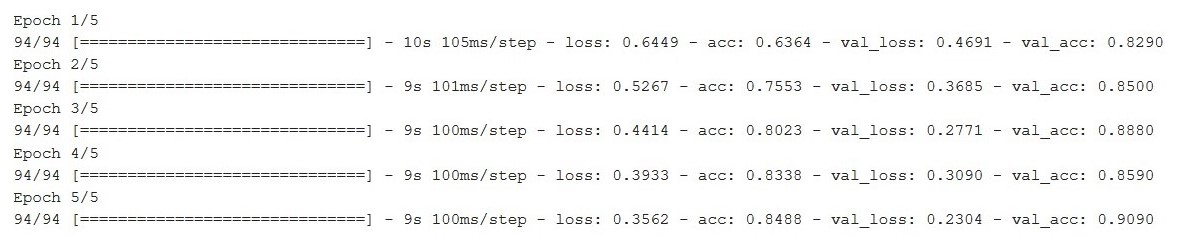
\includegraphics[scale = 0.63]{CHAPTERS/Chapter-4/Images/4.2}
    \caption{Training results for two class problem after 5 epochs} 
    \label{fig:4.2}
\end{figure}
\begin{figure}[H]
    \centering
    \captionsetup{justification = centering}
    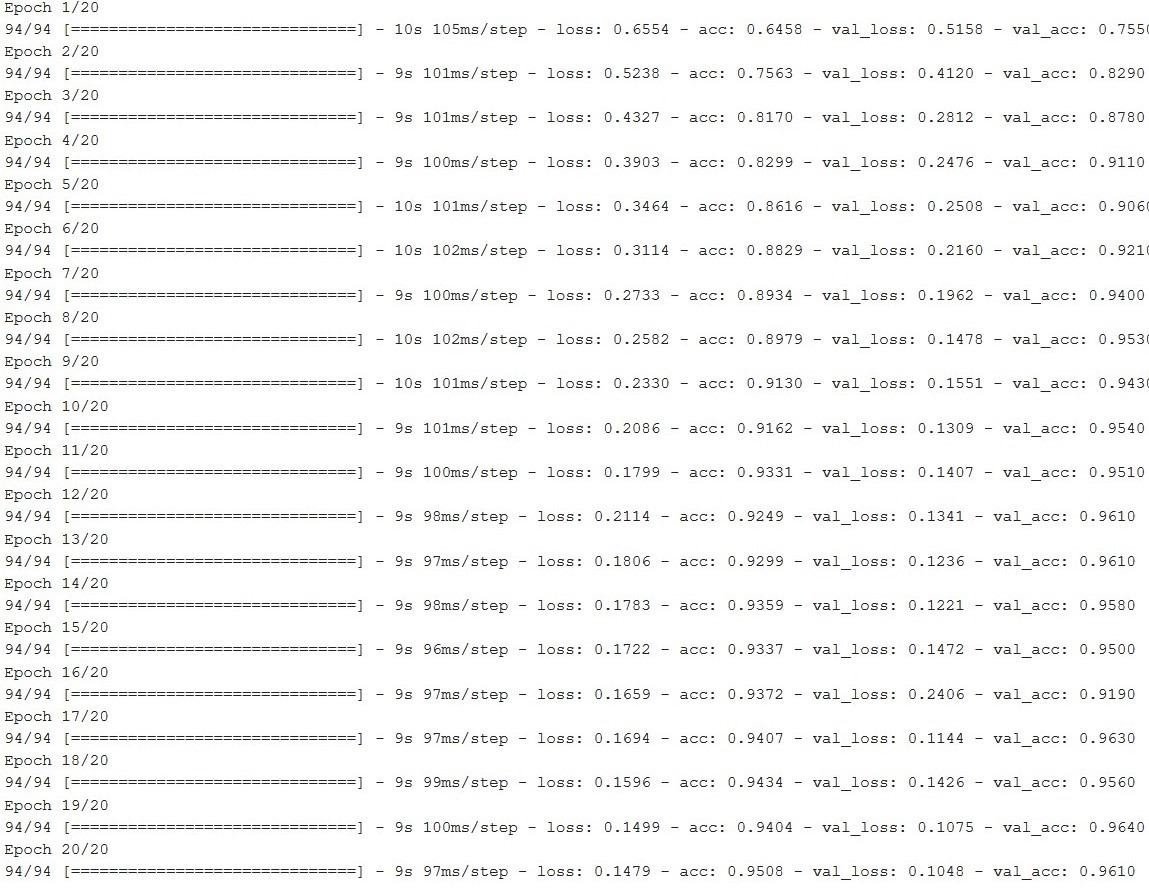
\includegraphics[scale = 0.63]{CHAPTERS/Chapter-4/Images/4.3}
    \caption{Training results for two class problem after 20 epochs} 
    \label{fig:4.3}
\end{figure}
After 20 epochs for this model, the validation loss increases which indicate
that we have to train that model up to 20 epochs. 

\subsection{Five Class Probem \& Results}
We started with two class problem and extended the model to five classes
which is our desired task. The loss function in this case is categorical\_crossentropy.
The model used for five class is a customized VGG-16. The details of the
model are shown in figure \ref{model_summary}.
\begin{figure}[H]
    \centering
    \captionsetup{justification = centering}
    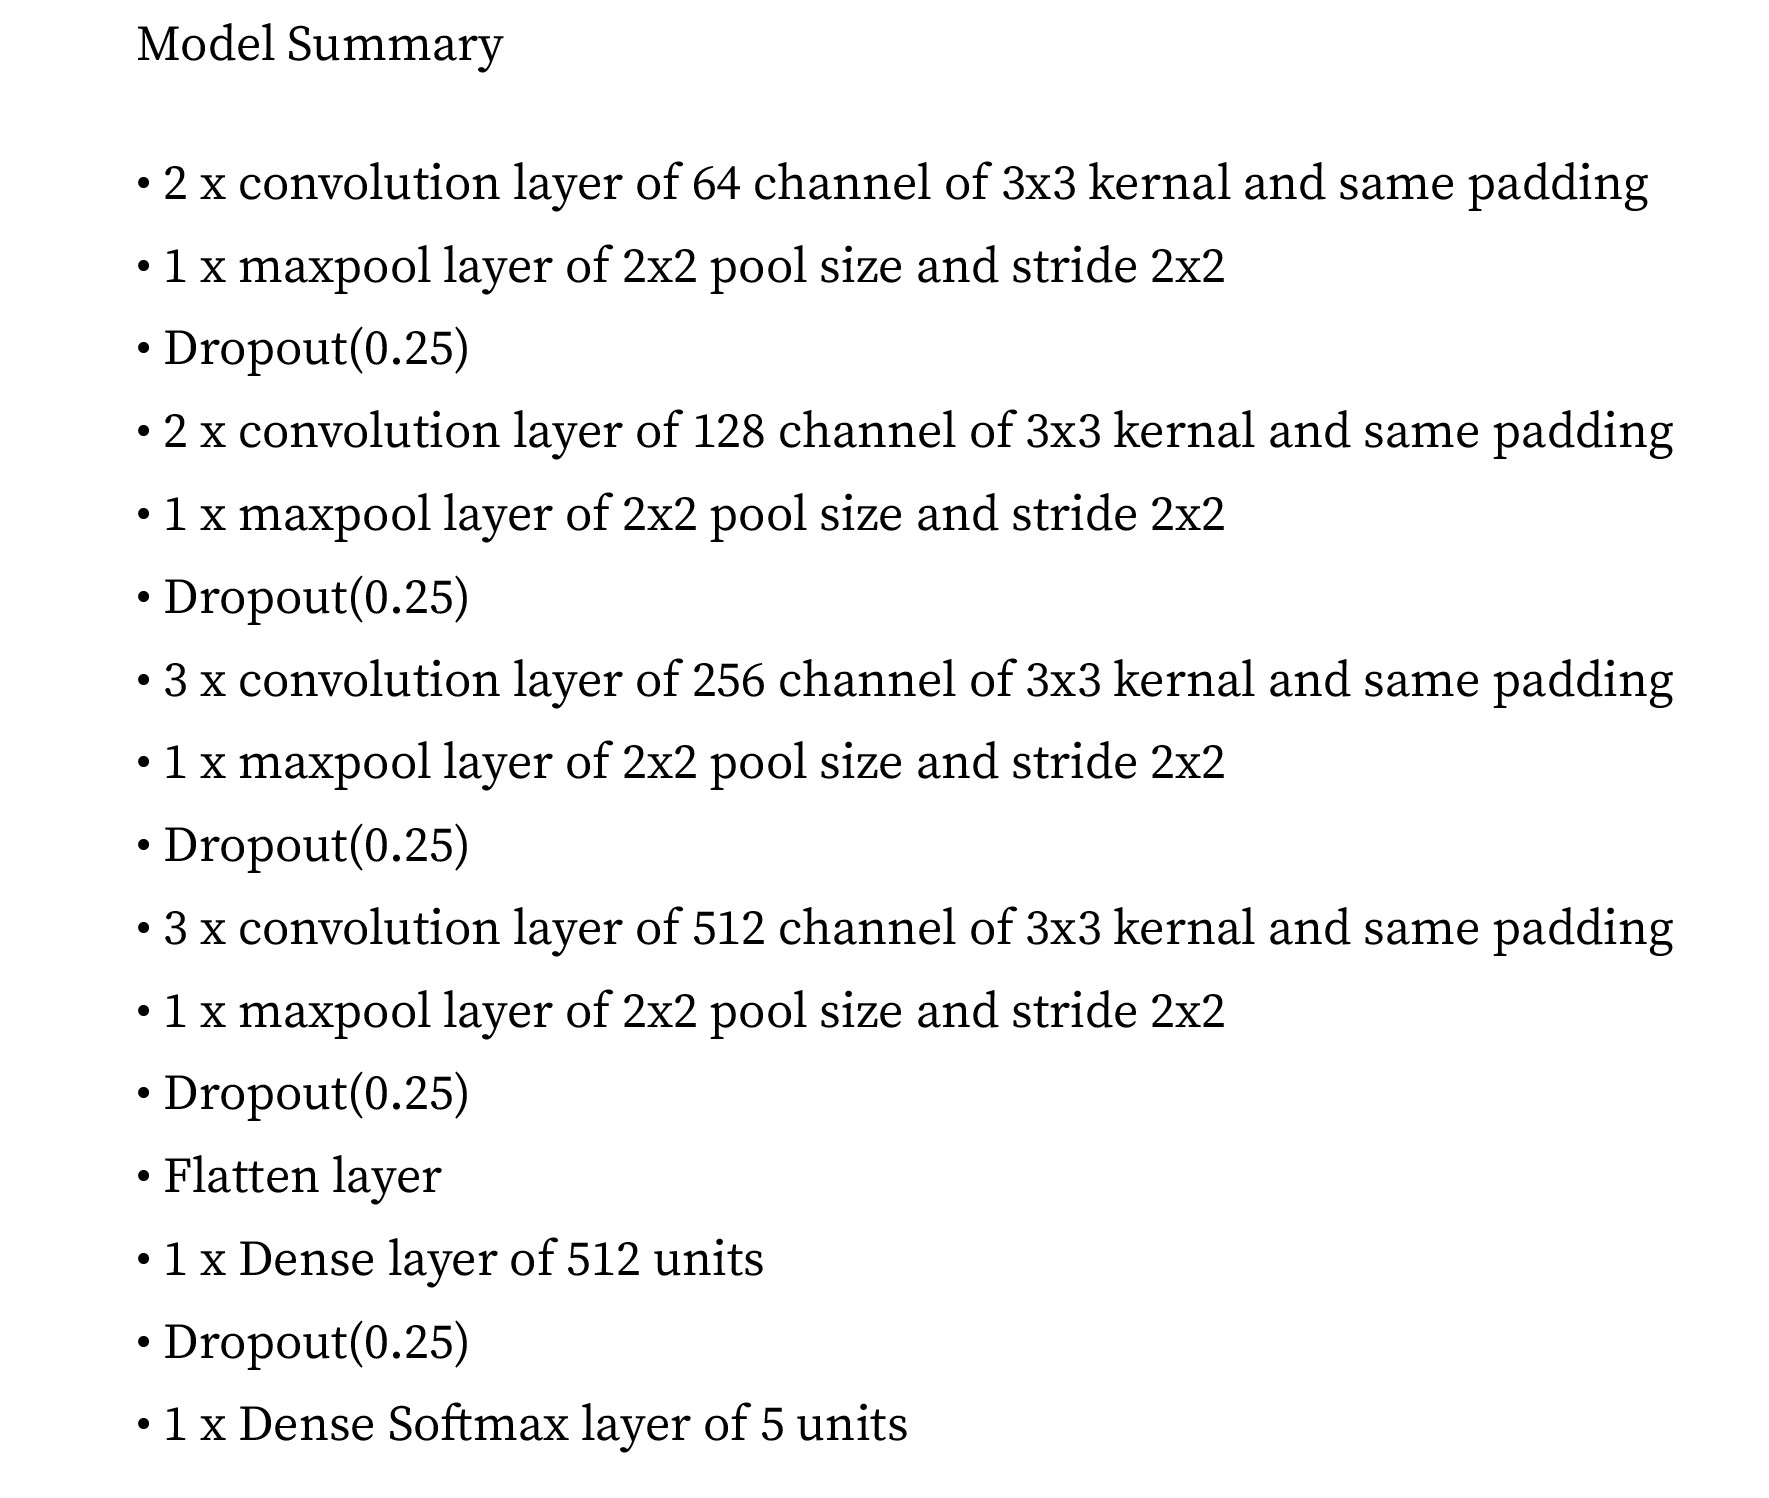
\includegraphics[scale = 0.8]{CHAPTERS/Chapter-4/Images/summary-01.jpg}
    \caption{Training results for two class problem after 20 epochs} 
    \label{model_summary}
\end{figure}
The optimizer used is RMSprop with
learning rate 0.0001. We started with 5 epochs, then 10 upto 20. The plot of training
and validation accuracy and training and validation loss is plotted using Python
matplotlib and it is observed that near to 20 the validation loss
increases and validation accuracy decreases. So we stopped at 20 epochs
and recorded the results. The plots are shown in
figure \ref{fig:4.4}.
\begin{figure}[htbp]
    \centering
    \begin{subfigure}[t]{0.45\textwidth}
        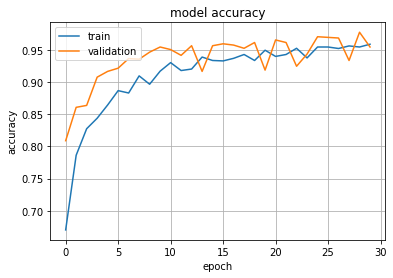
\includegraphics[scale = 0.52]{CHAPTERS/Chapter-4/Images/4.4a}
        \caption{Training \& validation accuracy}
        \label{fig:4.4a}
    \end{subfigure}
    \begin{subfigure}[t]{0.45\textwidth}
        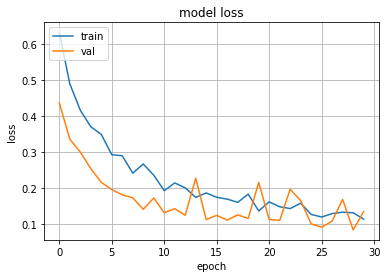
\includegraphics[scale = 0.52]{CHAPTERS/Chapter-4/Images/4.4b}
        \caption{Training \& validation loss}
        \label{fig:4.4b}
    \end{subfigure}
    \caption[]{Model accuracy \& model loss}
    \label{fig:4.4}
  \end{figure}
  The loss was binary\_crossentropy in this case. 
  The training accuracy recorded after 20 epochs was 93\% and training
  loss was 22.3\%. The test set was choosen as validation data and
  validation accuracy after 20 epochs 
  was 92.40\% and validation loss was 24\%.
  Here we attach the results only for 10 epochs and 20 epochs
  in figure \ref{fig:4.5} and \ref{fig:4.6}.
\begin{figure}[H]
    \centering
    \captionsetup{justification = centering}
    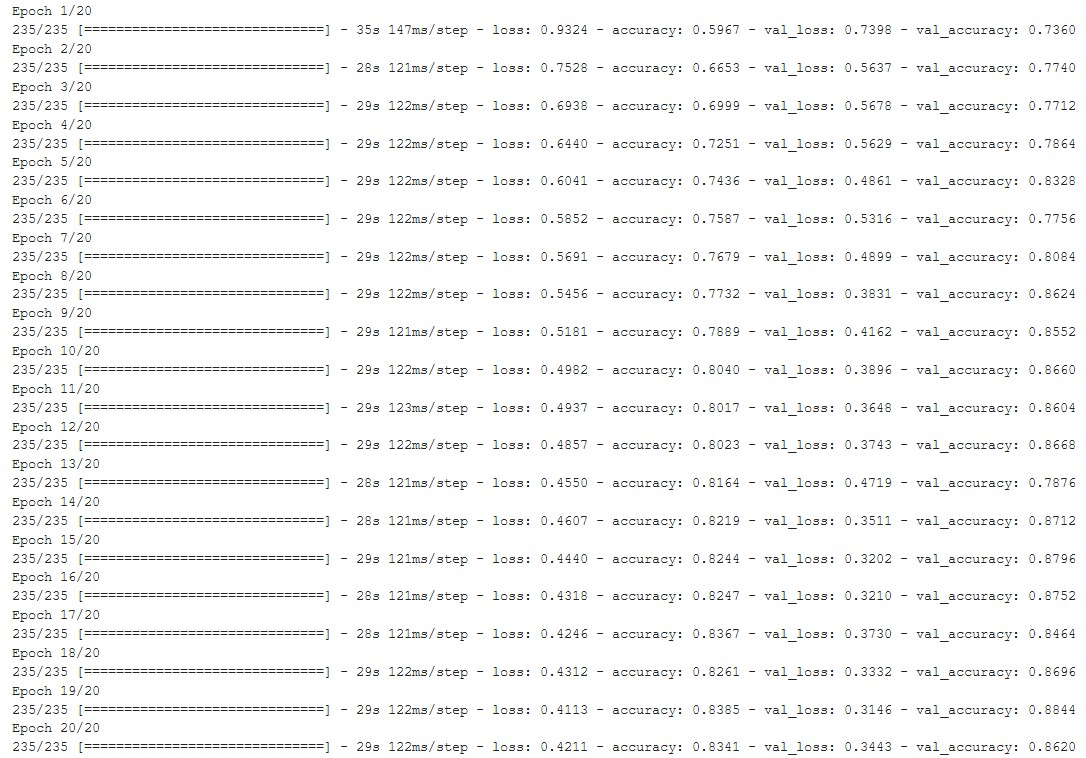
\includegraphics[scale = 0.53]{CHAPTERS/Chapter-4/Images/4.5}
    \caption{Training results for five class problem after 10 epochs} 
    \label{fig:4.5}
\end{figure}
\begin{figure}[H]
    \centering
    \captionsetup{justification = centering}
    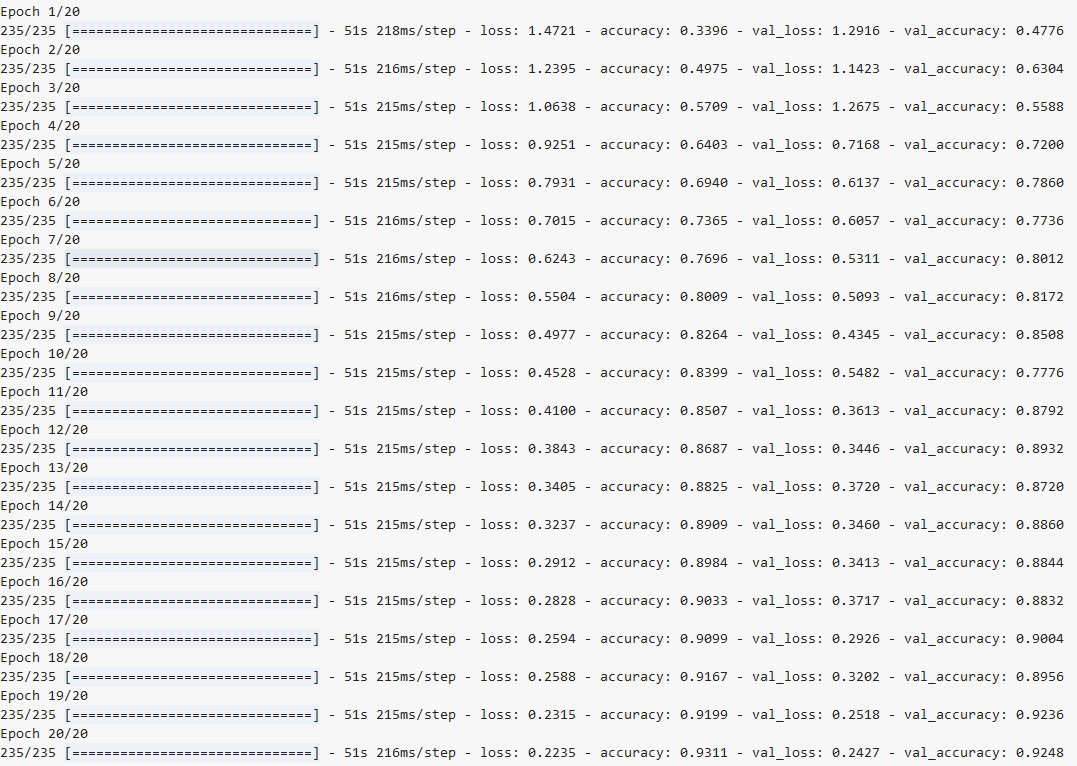
\includegraphics[scale = 0.68]{CHAPTERS/Chapter-4/Images/4.6}
    \caption{Training results for five class problem after 20 epochs} 
    \label{fig:4.6}
\end{figure}
\section{Graphical User Interface}
To observe the results in a concrete way, we have to pass test images
one by one and obtain the corresponding labels. For this purpose,
we made a Graphical User Interface (GUI) using tkinter package of Python.
As discussed earlier that we have saved the model in a folder named
as saved\_models in the root directory. This model can be downloaded to local
disks of the computer (As tkinter uses the GUI of computer, it can not
run on Colab). Then from the test directory, all the images one by one are passed
and corresponding labels are displayed. Some examples are shown in
figure \ref{fig:4.7}.

\begin{figure}[htbp]
    \centering
    \begin{subfigure}[t]{0.3\textwidth}
        \fbox{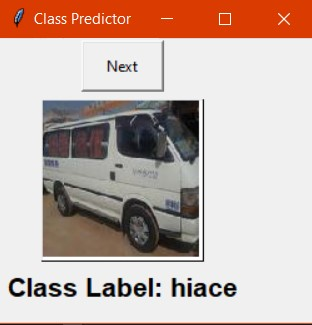
\includegraphics[width = 4.5cm, height = 4.5cm]{CHAPTERS/Chapter-4/Images/4.7a}}
        \caption{}
        \label{fig:4.7a}
    \end{subfigure}
    \begin{subfigure}[t]{0.3\textwidth}
        \fbox{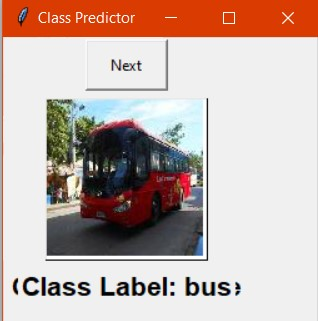
\includegraphics[width = 4.5cm, height = 4.5cm]{CHAPTERS/Chapter-4/Images/4.7b}}
        \caption{}
        \label{fig:4.7b}
    \end{subfigure}
    \begin{subfigure}[t]{0.3\textwidth}
      \fbox{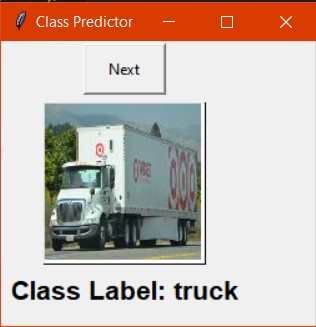
\includegraphics[width = 4.5cm, height = 4.5cm]{CHAPTERS/Chapter-4/Images/4.7c}}
      \caption{}
      \label{fig:4.7c}
  \end{subfigure}
    \captionsetup{justification = centering}
    \caption[]{Test images and labels on a GUI}
    \label{fig:4.7}
  \end{figure}

\section{Limitations \& Future Work}
This model does not work on high resolution images of two class problem.
For high class we use Res-Net architecture which is complex and
requires high computational power. We have used a variant of VGG-16 for
our five class problem. Highly complex model cause overfitting as model has
a minimal overfitting near 20 epochs. Moreover, hyperparameters tuning
plays an important role. Playing with the values of learning rate
and data can be recorded to have a detailed idea about the working
of various optimizers along with the variation of learning rate, exponential
decay etc. For future work, the detailed study about tuning of hyperparameters
is included.